\section{System Properties}

This section is used to outline and analyze the underlying system properties such as the hardware and software that was used for this project. 

\subsection{Hardware}

The distributed fashion of this project requires the use of multiple microcontrollers with access to wireless communication. 
To achieve this, a total number of four \texttt{(ESP 32-WROOM)} microcontrollers was chosen as the computational cluster.
This 32-bit chip offers \SI{520}{\kilo\byte} of RAM and a dual core architecture at \SI{240}{\mega\hertz}.
Additionally, it features a Wi-Fi antenna with a bit rate of up to \SI{150}{\mega\byte\per\second} aswell as a Bluetooth transmitter \cite{esp32_datasheet}. 
For this Wi-FI antenna, we conducted an experiment measuring the maximum possible distance for data exchange. 
While various different sources suggest a range of more than \SI{200}{\meter}, the connection in our case, however, was lost after only \SI{15.6}{\meter}.
For the interaction with the controlled cluster, it allows access to 32 GPIO pins with different capabilities. 
The layout and design of the used board is visible in Figure \ref*{fig:esp32_pinout}.

\begin{figure}[htbp]
    \centering
    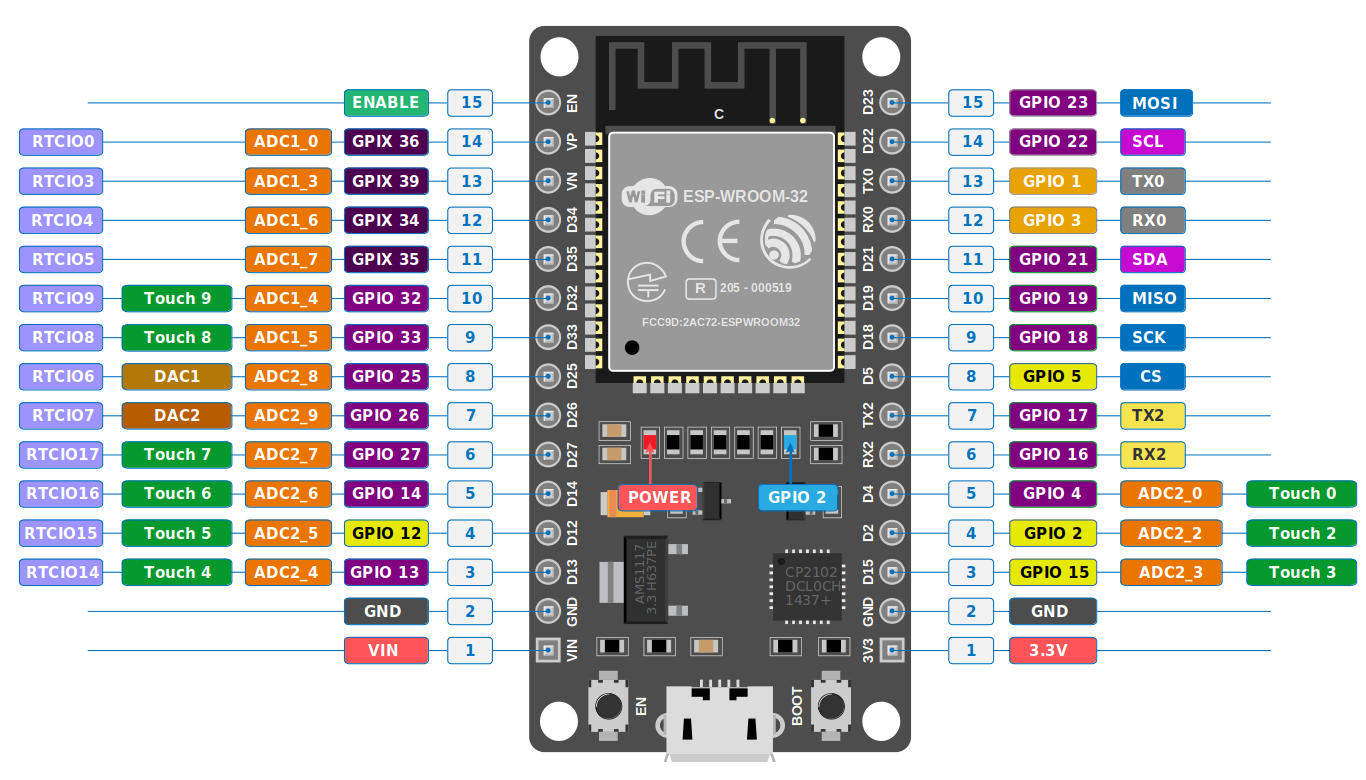
\includegraphics[width=0.8\textwidth]{images/esp_layout.png}
    \caption{Pinout diagram of the ESP32-WROOM module \cite{pinout_diagram}.}
    \label{fig:esp32_pinout}
\end{figure}

To display the current state of each traffic light, multiple prebuilt LED modules \ref*{fig:ampel_module} were used for simplicity. 
Each of them features a red, yellow and green LED, that can each be individually controlled using an input at the base of the module. 
The method of output can be freely chosen and even set up to function with real-world traffic lights
As an additional output the AMPEL can use a 4-digit 7-segment \texttt{TM1637} display \ref*{fig:display} to show numbers and ASCII characters. 
This external module can be configured using a 4-pin interface that allows for a continuous data flow to the display. 

\begin{figure}[htbp]
     \centering
     \begin{subfigure}[b]{0.45\textwidth}
         \centering
         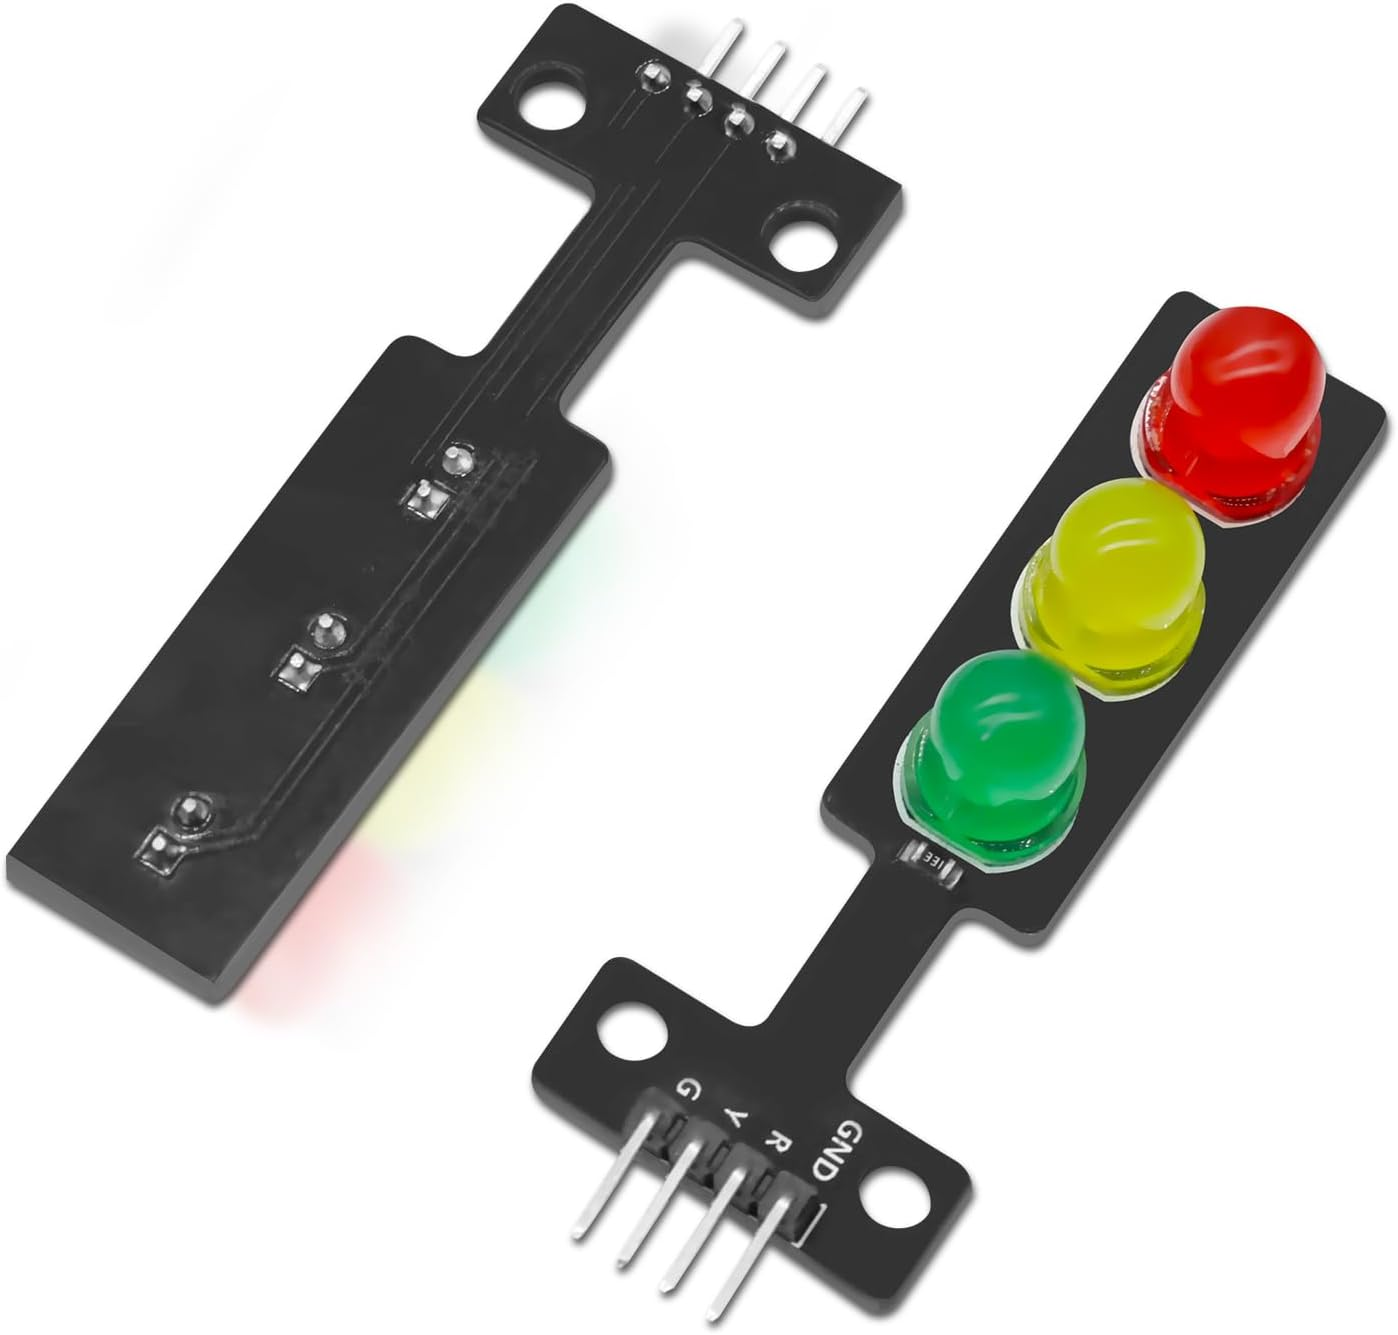
\includegraphics[width=0.75\textwidth]{images/ampel.jpg}
         \caption{Traffic light module}
         \label{fig:ampel_module}
     \end{subfigure}
     \hfill
     \begin{subfigure}[b]{0.45\textwidth}
         \centering
         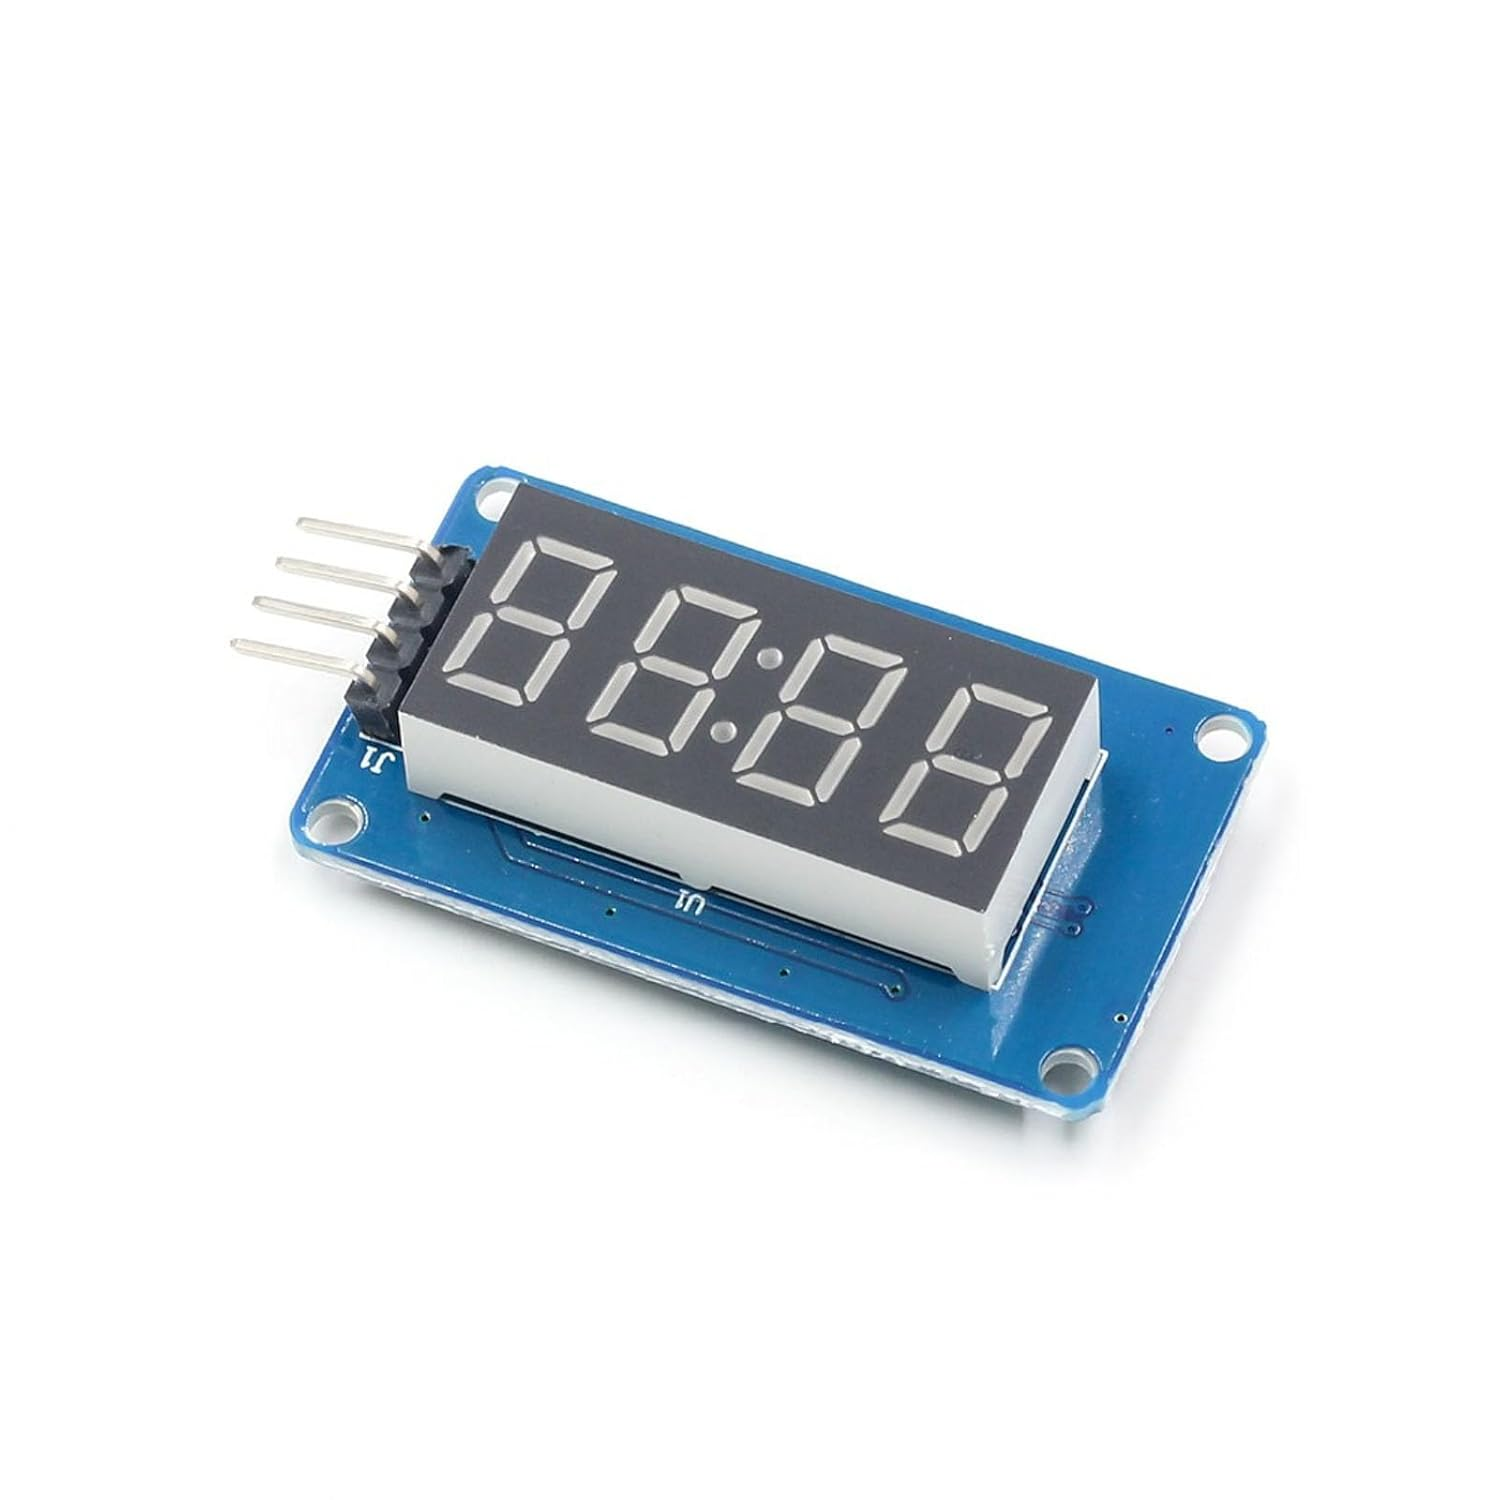
\includegraphics[width=0.75\textwidth]{images/display.jpg}
         \caption{7 segment display}
         \label{fig:display}
     \end{subfigure}
     \caption{External ESP modules}
     \label{fig:modules}
\end{figure}

\subsection{Software}

The program that is running on the Espressif microcontrollers was created on the basis of the \texttt{ESP-IDF} framework using the PlatformIO development platform.
This program is compiled and flashed from a \texttt{C} codebase and afterwards executed using the \texttt{FreeRTOS} operating system for real-time systems.
FreeRTOS supplies the possibility to use threads and other concurrent execution utilities, which are crucial for the parallel output and communication capabilities of the AMPEL.
It additionally includes timing capabilities that are used to effectively schedule tasks to be executed at a set timestamp.

The communication between the ensemble of microcontrollers is handled by \texttt{ESP-Now}, which is a connectionless peer-to-peer protocol for wireless communication over Wifi.
The exchanges of messages do therefore not require any intermediate router and no actual WLAN-Handshake is required for the connection.
Data is also directly exchanged on the Data Link Layer, which results in a ultra-low overhead compared to a usual TCP/IP connection.
The transmission latency of an ESP-Now connection is very short compared to TCP/IP connections with a measured latency of under \SI{2}{\milli\second}.
ESP-Now can be used for both broadcasting and unicasting messages at a maximum packet size of \SI{250}{\byte}.

The ESP-IDF library for interaction with ESP-NOW acts as a very simple interface to sending and receiving data, but also as a store for current peers.
The sending is handled by the library function \texttt{esp\_now\_send()}, which requires the MAC address of the recipient and the data as an input. 
Once this packet is transmitted from the WIFI interface, it triggers a \texttt{on\_send} callback function that can be used to accurately detect lost packets and other metrics. 
A similar callback is triggered, when a node receives a packet. 

The controlling of the 7-segment display \ref*{fig:display} is handled by a ESP-IDF driver \cite{esp_idf_tm1637} for TM1637.
This driver can be used to send simple instructions containing just the number or string that should be shown without requiring a more granular interaction with the onboard pins. 

